\documentclass[a4paper,14pt]{extarticle}
%\documentclass[a4paper]{article}
\usepackage[T2A]{fontenc}
\usepackage[utf8]{inputenc}
\usepackage[english,russian]{babel}
\usepackage{indentfirst}
\usepackage{amssymb}
\usepackage{amsfonts}
\usepackage{amsmath}
\usepackage{mathtext}
\usepackage{cite}
\usepackage{enumerate}
\usepackage{float}
\usepackage[top=1.5cm,bottom=1.5cm,left=2.5cm,right=1.5cm]{geometry}
\usepackage[unicode]{hyperref}
\usepackage{graphicx}
\usepackage{color}
\usepackage[colorinlistoftodos]{todonotes}
\usepackage[format=hang, labelsep=period, margin=10pt, figurename=Рис.]{caption}
\usepackage{listings}
\usepackage{subcaption}
%\usepackage{showkeys}
\usepackage[onehalfspacing]{setspace}

\hyphenation{объёмом}
\hyphenpenalty=2000

\definecolor{dkgreen}{rgb}{0,0.6,0}
\definecolor{gray}{rgb}{0.5,0.5,0.5}
\definecolor{mauve}{rgb}{0.58,0,0.82}
 
\lstset{ %
  language=C++,                % the language of the code
  basicstyle=\footnotesize,           % the size of the fonts that are used for the code
%  numbers=left,                   % where to put the line-numbers
%  numberstyle=\tiny\color{gray},  % the style that is used for the line-numbers
%  stepnumber=2,                   % the step between two line-numbers. If it's 1, each line 
                                  % will be numbered
  numbersep=5pt,                  % how far the line-numbers are from the code
  backgroundcolor=\color{white},      % choose the background color. You must add \usepackage{color}
  showspaces=false,               % show spaces adding particular underscores
  showstringspaces=false,         % underline spaces within strings
  showtabs=false,                 % show tabs within strings adding particular underscores
  frame=single,                   % adds a frame around the code
  rulecolor=\color{black},        % if not set, the frame-color may be changed on line-breaks within not-black text (e.g. commens (green here))
  tabsize=2,                      % sets default tabsize to 2 spaces
  captionpos=b,                   % sets the caption-position to bottom
  breaklines=true,                % sets automatic line breaking
  breakatwhitespace=false,        % sets if automatic breaks should only happen at whitespace
  title=\lstname,                   % show the filename of files included with \lstinputlisting;
                                  % also try caption instead of title
  keywordstyle=\color{blue},          % keyword style
  commentstyle=\color{dkgreen},       % comment style
  stringstyle=\color{mauve},         % string literal style
  escapeinside={\%*}{*)},            % if you want to add a comment within your code
  morekeywords={*,...}               % if you want to add more keywords to the set
}
\renewcommand\lstlistingname{Листинг}
\renewcommand\lstlistlistingname{Листинги}
\newcommand{\itodo}{\todo[inline]}
\lstloadlanguages{C++}
\DeclareCaptionFont{blue}{\color{blue}} 
%\%captionsetup[lstlisting]{singlelinecheck=false, labelfont={blue}, textfont={blue}}
%\DeclareCaptionFont{white}{\color{white}}
%\DeclareCaptionFormat{listing}{\colorbox[cmyk]{0.43, 0.35, 0.35,0.01}{\parbox{\textwidth}{\hspace{15pt}#1#2#3}}}
%\captionsetup[lstlisting]{
%	format=listing,
%	labelfont=white,
%	textfont=white,
%	singlelinecheck=false,
%	margin=0pt,
%	font={bf,footnotesize}
%}
\numberwithin{equation}{section}
\setcounter{secnumdepth}{3} % глубина нумеруемых разделов
\setcounter{tocdepth}{3} % глубина оглавления
\begin{document}
%\listoftodos
%\clearpage
\newpage
\begin{titlepage}
\newpage

\begin{center}
ФЕДЕРАЛЬНОЕ АГЕНТСТВО ПО ОБРАЗОВАНИЮ\\РОССИЙСКОЙ ФЕДЕРАЦИИ\\
Государственное образовательное учреждение высшего профессионального образования\\
\textbf{Национальный исследовательский ядерный университет <<МИФИ>>}\\
\hrulefill\\
ФАКУЛЬТЕТ ЭКСПЕРИМЕНТАЛЬНОЙ И\\ТЕОРЕТИЧЕСКОЙ ФИЗИКИ\\
\vspace{1cm}
КАФЕДРА №31 <<ПРИКЛАДНАЯ МАТЕМАТИКА>>\\
\end{center}

\vspace{8em}

\begin{center}
\Large Пояснительная записка к дипломной работе на тему:
\end{center}

\vspace{2.5em}

\begin{center}
\textsc{\textbf{Численное моделирование низкоскоростного удара по многослойной инженерной конструкции}}
\end{center}

\vspace{6em}

\begin{flushleft}
\vspace{1.5em}
Студент-дипломник \hrulefill Ермаков А.С.\\
\vspace{1.5em}
Научный руководитель \hrulefill д.ф.-м.н. проф. Петров И.Б.\\
\vspace{1.5em}
Рецензент \hrulefill \\
\vspace{1.5em}
Заведующий кафедров №31\hrulefill д.ф.-м.н. проф. Кудряшов Н.А.\\
\end{flushleft}

\vspace{\fill}
\begin{center}
Москва 2012
\end{center}

\end{titlepage}

\tableofcontents
\clearpage
\newpage
\section*{Введение}
\addcontentsline{toc}{section}{Введение}
В данной работе рассматривается метод численного моделирования низкоскоростного
удара по многослойной инженерной конструкции. Под низкоскоростным ударом
понимается такое столкновение двух тел, при котором не происходит заметных
деформаций.

Многослойные конструкции нашли применение во многих технических областях. Одним
из самых ярких примеров являются композиционные материалы -- искусственно
созданные  материалы, состоящие из нескольких слоёв с чёткой границей раздела
между ними. Композиционные материалы используются в авиации и космонавтике: они
применяются для изготовления обшивок воздушных и космических аппаратов, а также
при создании силовых конструкций, испытывающих серьёзные нагрузки. Композитные
материалы одновременно обладают лёгкостью и заметной прочностью, поэтому всё
чаще они используются для создания брони военной техники и бронежилетов.
Преградой на пути к массовому использованию композиционных материалов является
отсутствие экспериментальных методов проверки характеристик таких материалов.
Так, давно опробованные и использующиеся методы измерения прочностн\'{ы}х
характеристик металлов, не подходят для анализа композитов: композиты по своей
природе анизотропны.

Одной из актуальных прикладных задач, связанных с испытанием многослойных
материалов, является задача о получении волновой картины в образце после
непробивающего удара. В силу анизотропности свойств многослойные материалы после
нагрузок могут заметно терять прочность даже при отсутствии видимых поврежедний.
Это обусловлено появлением микротрещин, которые впоследствии, объединяясь,
превращаются в макротрещины. Так, возникающее после нагрузки расслоение
материала может быть визуально не заметно, хотя делает образец непригодным к
дальнейшему использованию.

Поведение композиционных материалов при динамических нагрузках хорошо
описывается уравнениями механики деформируемого твёрдого тела. Решить эти
уравнения аналитически в большинстве случаев не представляется возможным ввиду
сложности геометрии подобных задач. Поэтому в последнее время для испытания
композиционных материалов используют следующий подход:
\begin{itemize}
\item проводят эксперимент по нагружению опытного образца;
\item моделируют этот эксперимент численно;
\item проводят валидацию результатов моделирования значениями, полученными в ходе эксперимента;
\item при прохождении проверки используют результаты численного моделирования
для получения картины динамической деформации образца.
\end{itemize}

На данный момент в открытом доступе нет программ численного моделирования, в
основе которых лежит сеточно-характеристический метод. При этом сам метод 
обладает рядом достоинств (к примеру, в отличие от многих используемых алгортимов
возможно явное выделение контактной границы) и в теории должен давать весьма
качественные результаты. Поэтому в данной работе предпринята попытка реализации
программного комплекса для высокопроизводительных вычислений в области механики
деформируемого твёрдого тела с использованием сеточно-характеристического
метода.

\clearpage
\newpage
\subsection*{Постановка задачи}
\addcontentsline{toc}{subsection}{Постановка задачи}
\begin{figure}[h]
\center{\includegraphics[width=\textwidth]{png/construction.png}}
\caption{Обшивка и силовой кессон крыла.}
\label{pic:construction}
\end{figure}
Одной из практических задач о динамическом нагружении композиционных материалов
является задача о непробивающем ударе по обшивке крыла самолёта. На рис.
\ref{pic:construction} приведена схема строения обшивки и силового кессона
крыла, выполненных из композиционных материалов. Обшивка толщиной 6.5~мм состоит 
из 3 композитных субпакетов, соединенных между собой эпоксидной смолой, 
а стрингер толщиной 13~мм -- из 6 аналогичных субпакетов. Каждый субпакет
состоит из 11 монослоёв со взаимной ориентацией субпакетов при укладке 
45/0/-45/0/0/90/0/0/-45/0/45. Каждый монослой имеет следующий состав: 60\% -- 
ориентированные длинные углепластиковые волокна; 40\% -- матрица
(эпоксидная смола). 

Ввиду большой вычислительной сложности при моделировании подобной конструкции с 
точностью до отдельного волокна, а также из-за многообразия протекающих процессов, 
полная задача декомпозируется на ряд подзадач. В данной работе рассматривается задача о получении
волновой картины в элементе композитной обшивки крыла при следующих условиях:
\begin{itemize}
\item обшивка состоит из трёх субпакетов, сооединённых эпоксидной смолой;
\item каждый субпакет изотропен по своим свойствам;
\item толщина субпакетов и соединяющих эпоксидных слоёв одинакова;
\item размеры одного субпакета: 20x20x1~мм.
\end{itemize}
Упругие характеристики слоёв приведены в табл. \ref{tbl:subpackage}
\begin{table}
\centering
\begin{tabular}{|c|c|c|c|c|c|c|c|}
\hline
Слой & E, ГПа & $\nu$ & $\rho$, кг/м$^{3}$ & $\lambda$, ГПа & $\mu$, ГПа &
$c_p$, м/с & $c_s$, м/с \\
\hline
Эпоксидная смола & 2.5 & 0.3 & 1250 & 1.44 & 0.96 & 1640 & 876 \\
Субпакет & 8 & 0.3 & 1250 & 4.62 & 3.08 & 2937 & 1570 \\
\hline
\end{tabular}
\caption{Упругие характеристики слоёв.}
\label{tbl:subpackage}
\end{table}
Эти параметры в изотропном приближении моделируют обшивку крыла самолёта и
позволяют качественно получить волновую картину после непробивающего удара.

В эксперименте по непробивающему воздействию на обшивку нагрузка создается 
металлическим ударником диаметром 25.4~мм. Характерный пример профиля нагрузки 
при испытаниях приведен на рис. \ref{pic:loadprofile}. Давление на поверхности 
крыла в ходе эксперимента находится в диапазоне 0-100~МПа. Поэтому для численного 
моделирования выбирается воздействие с давлением 50~МПа.
\begin{figure}[h]
\center{\includegraphics[width=\textwidth]{png/load-profile.png}}
\caption{Пример профиля нагрузки на обшивку крыла при испытаниях.}
\label{pic:loadprofile}
\end{figure}

Резюмируя, можно выделить следующие цели работы:
\begin{itemize}
\item предложить алгоритм построения параллельной версии сеточно"=характеристического метода в случае трёх пространственных переменных на неструктурированных сетках;
\item реализовать предложенный алгоритм в виде программного комплекса;
\item получить волновую картину в обшивке после низкоскоростного удара при
указаных выше допущениях.
\end{itemize}

\subsection*{Существующие работы на схожую тематику}
\addcontentsline{toc}{subsection}{Существующие работы на схожую тематику}

Для динамических задач механики деформируемого твердого тела необходимо использование численных методов, позволяющих получить полную волновую картину с высоким временным и пространственным разрешением с учётом влияния контактных границ. Так как определяющая система уравнений в частных производных относится к гиперболическому типу, одними из наиболее широко используемых вычислительных методов для её решения являются сеточно-характеристические методы, подробное описание и обзор которых можно найти в \cite{magomedov}. Существенное продвижение было получено в работах \cite{chushkin}, основанных на сочетании метода характеристик и конечно-разностных подходов.

В работе \cite{petrov_chelnokov} рассматриваются особенности протекания процессов деформирования в многослойных преградах конечной толщины, вызванных ударом абсолютно твёрдого сферического тела. Для моделирования поведения материала преграды использовались реологические модели линейно-упругой среды (закон Гука), упругопластической (модель Прандтля-Рейса с условиями пластичности Мизеса и Мизеса-Шлейхера, модель Максвелла), упруговязкопластической сред. Характерной особенностью работы является использование модели разрушения (модель Майнчена-Сака), а также использование различных подходов к перестроению сеток. Для численного решения использовался сеточно-характеристический метод, гибридная и гибридизованная разностные схемы. Минусами является использование структурированной (прямоугольной) сетки и только двух пространственных переменных.

В работе \cite{matyushev_petrov} проводилось численное исследование волновых и деформационных процессов в многослойных  средах. Как и в предыдущей работе, использовался численно-характеристический метод, а также гибридная и гибридизированная схемы. Особенностью является использование неструктурированных (треугольных) сеток, а также применение сеточно-характеристического шаблона на неструктурированных сетках (этот подход нетипичен для данного метода, так как использование шаблона предполагает наличие структурированной сетки). Моделировался удар деформируемым сферическим ударником по многослойной (5 – 20 слоев) преграде. Данная модель описывала бронежилет и человеческое тело, защищённое им. Целью было найти оптимальные параметры среды для максимального поглощения воздействия ударника. К недостаткам работы можно отнести моделирование лишь по двум пространственным координатам.

В \cite{petrov_tormasov_holodov} рассмотрены одномерные и двумерные нестационарные задачи о действии ударных нагрузок на деформируемые твёрдые среды многослойной структуры, описаны возникающие волновые эффекты, приводящие к появлению откола. Для описания поведения среды использованы модели линейно упругого и упругоидеальнопластического тела. На поверхностях раздела слоев рассматрены условия трёх типов: полного слипания, свободного скольжения, отслоения. В работе изучалось в основном влияние многослойных структур на амплитуду проходящей волны. На основании одномерных расчётов в слоистых средах был сделан вывод, что слоистые конструкции можно использовать для уменьшения амплитуды волн и для увеличения сжимающих напряжений вблизи лицевой поверхности, например, для увеличения силы сопротивления.

В \cite{golubev_kvasov_petrov} исследуются задачи распространения упругих волн, возникающих в результате землетрясения, в различных геологических средах: однородной, многослойной, градиентной, с трещиноватым пластом и карстовым образованием. Также проводится анализ воздействия упругих волн на поверхностные промышленные сооружения: здания и плотины. Проводится сравнение воздействия упругих волн на дневную поверхность для различных геологических сред. Качественно рассматривается влияние упругих волн на прочность поверхностных сооружений. В работе используется сеточно"=характеристический метод на треугольных сетках, контактные границы выделяются явно.

В \cite{agapov_belocerkovsky_petrov} сформулирована двумерная математическая модель механической реакции головы человека на ударные воздействия, описывающая пространственное распределение механических нагрузок на мозг (система череп-мозг с точки зрения механики также является многослойной средой). Приведены некоторые результаты ее численного исследования с применением сеточно-характеристических методов на структурированных (прямоугольных) и неструктурированных (треугольных) сетках.

Работа \cite{petrov} посвящена численному исследованию волновых процессов и явления откола, возникающих при импульсном нагружении двух- и четырехслойных упругопластических цилиндрических оболочек конечной толщины, подкрепленных с тыльной стороны ребрами жесткости. Используется динамическая система двумерных уравнений механики деформируемого тела и упруго идеально пластическая модель Прандтля-Рейсса. В работе показана возможность не только получать разрушенные зоны, но и отдельные трещины, зоны концентраций напряжений вблизи трещины и края откольной зоны, которая переходит в трещину, являющуюся самостоятельным источником нестационарных возмущений.

Автору не известны работы на схожую тематику, использующие сеточно-характеристический метод на неструктурированных сетках при трех пространственных переменных с явным выделением контактных границ.


\clearpage
\newpage
\section{Уравнения механики деформируемого твёрдого тела}
\subsection{Уравнения движения и реологические соотношения}
Для математического моделирования волновых процессов в деформируемом твёрдом
теле используется система динамических уравнений \cite{novatsky,sedov} в виде
\begin{eqnarray}
\label{rheology_equations}
\rho\dot{v}_i=\nabla_j\sigma_{ij}+f_i & \textrm{(уравнения движения)}\nonumber\\
\dot{\sigma}_{ij}=q_{ijkl}\dot{\varepsilon}_{kl}+F_{ij} & \textrm{(реологические
соотношения).}
\end{eqnarray}

Здесь $\rho$ – плотность среды, $v_i$ – компоненты скорости смещения,
$\sigma_{ij}$, $\varepsilon_{ij}$ -- компоненты тензоров напряжений и деформаций,
$\nabla_j$ – ковариантная производная по $j$-й координате, $f_i$ – массовые
силы, действующие на единицу объёма, $F_{ij}$ -- добавочная правая часть.

В случае малых деформаций тензор скоростей деформаций $e_{ij}=\dot{\varepsilon}_{ij}$ 
выражается через компоненты скорости смещения линейным образом:
\begin{equation}
e_{ij}=\frac{1}{2}(\nabla_j v_i+\nabla_i v_j).
\end{equation}
Вид компонент тензора 4-го порядка $q_{ijkl}$ определяется реологией среды. Для 
линейно-упругого тела
\begin{eqnarray}
\label{tensor_qijkl}
q_{ijkl}=\lambda\delta_{ij}\delta_{kl}+\mu(\delta_{ik}\delta_{jl}+\delta_{il}
\delta_{jk}),\nonumber\\
F_{ij}=0.
\end{eqnarray}
В этом соотношении, которое обобщает закон Гука, $\lambda$ и $\mu$ -- параметры
Ляме, $\delta_{ij}$ -- символ Кронекера.

Для замыкания системы уравнений \ref{rheology_equations} её необходимо дополнить
уравнением состояния, определяющим зависимость плотности от напряжений:
$$\rho=\rho_0e^{\frac{p}{K}},$$
где $p=-\frac{1}{3}\sum\sigma_{kk}$ -- давление, $K=\lambda+\frac{2}{3}\mu$ --
коэффициент всестороннего сжатия.
\subsection{Матричная форма уравнений}
Уравнения \ref{rheology_equations} и \ref{tensor_qijkl} можно переписать в матричной
форме:
\begin{equation}
\label{matrix_equation}
\frac{\partial}{\partial{t}}\vec{u}^T+\mathbf{A}_x\frac{\partial}{\partial{x}}\vec{u}^T+
\mathbf{A}_y\frac{\partial}{\partial{y}}\vec{u}^T+
\mathbf{A}_z\frac{\partial}{\partial{z}}\vec{u}^T=\vec{f}^T.
\end{equation}
Здесь
$\vec{u}=\{v_x,v_y,v_z,\sigma_{xx},\sigma_{yy},\sigma_{zz},\sigma_{xy},\sigma_{xz},\sigma_{yz}\}$
-- вектор искомых функций, $\vec{f}$ -- вектор правых частей той же размерности,
$x,y,z$ --  независимые пространственные переменные, $t$ -- время,
\begin{displaymath}
\mathbf{A}_x =
\left( \begin{array}{cccccccccccc}
0 & 0 & 0 & -\frac 1 \rho & 0 & 0 & 0 & 0 & 0 \\ 
0 & 0 & 0 & 0 & -\frac 1 \rho & 0 & 0 & 0 & 0 \\ 
0 & 0 & 0 & 0 & 0 & -\frac 1 \rho & 0 & 0 & 0 \\ 
-\lambda-2\mu & 0 & 0 & 0 & 0 & 0 & 0 & 0 & 0 \\ 
0 & -\mu & 0 & 0 & 0 & 0 & 0 & 0 & 0 \\ 
0 & 0 & -\mu & 0 & 0 & 0 & 0 & 0 & 0 \\ 
-\lambda & 0 & 0 & 0 & 0 & 0 & 0 & 0 & 0 \\ 
0 & 0 & 0 & 0 & 0 & 0 & 0 & 0 & 0 \\ 
-\lambda & 0 & 0 & 0 & 0 & 0 & 0 & 0 & 0  
\end{array} \right),
\end{displaymath} 
\begin{displaymath}
\mathbf{A}_y =
\left( \begin{array}{cccccccccccc}
0 & 0 & 0 & 0 & -\frac 1 \rho & 0 & 0 & 0 & 0 \\ 
0 & 0 & 0 & 0 & 0 & 0 & -\frac 1 \rho & 0 & 0 \\ 
0 & 0 & 0 & 0 & 0 & 0 & 0 & -\frac 1 \rho & 0 \\ 
0 & -\lambda & 0 & 0 & 0 & 0 & 0 & 0 & 0 \\ 
-\mu & 0 & 0 & 0 & 0 & 0 & 0 & 0 & 0 \\ 
0 & 0 & 0 & 0 & 0 & 0 & 0 & 0 & 0 \\ 
0 & -\lambda-2\mu & 0 & 0 & 0 & 0 & 0 & 0 & 0 \\ 
0 & 0 & -\mu & 0 & 0 & 0 & 0 & 0 & 0 \\ 
0 & -\lambda & 0 & 0 & 0 & 0 & 0 & 0 & 0  
\end{array} \right),
\end{displaymath}
\begin{displaymath}
\mathbf{A}_z =
\left( \begin{array}{cccccccccccc}
0 & 0 & 0 & -\frac 1 \rho & 0 & 0 & 0 & 0 & 0 \\ 
0 & 0 & 0 & 0 & -\frac 1 \rho & 0 & 0 & 0 & 0 \\ 
0 & 0 & 0 & 0 & 0 & -\frac 1 \rho & 0 & 0 & 0 \\ 
-\lambda-2\mu & 0 & 0 & 0 & 0 & 0 & 0 & 0 & 0 \\ 
0 & -\mu & 0 & 0 & 0 & 0 & 0 & 0 & 0 \\ 
0 & 0 & -\mu & 0 & 0 & 0 & 0 & 0 & 0 \\ 
-\lambda & 0 & 0 & 0 & 0 & 0 & 0 & 0 & 0 \\ 
0 & 0 & 0 & 0 & 0 & 0 & 0 & 0 & 0 \\ 
-\lambda & 0 & 0 & 0 & 0 & 0 & 0 & 0 & 0  
\end{array} \right).
\end{displaymath}
\subsection{Гиперболические свойства систем уравнений линейной упругости}
Рассмотрим одномерное уравнение вида
\begin{equation}
\frac{\partial}{\partial{t}}\vec{u}^T+\mathbf{A}\frac{\partial}{\partial{x}}\vec{u}^T=\vec{f}^T.
\label{advection_equation}
\end{equation}
Если матрица $\mathbf{A}$ имеет полный набор вещественных собственных значений, 
то такое уравнение называется гиперболическим, и его решения соответствуют 
процессам, которые носят волновой характер. В этом случае справедливо разложение:
$$\mathbf{A}=\mathbf\Omega^{-1}\mathbf\Lambda\mathbf\Omega,$$
где $\mathbf\Omega$ -- матрица, составленная из векторов ${\vec\omega_i}$, где
$\vec\omega_i$ есть собственные векторы матрицы $\mathbf A$,
удовлетворяющие соотношениям
$$\vec\omega_i\mathbf A=\lambda_i\vec\omega_i,$$
а $\mathbf\Lambda=diag\{\lambda_i\}$ -- диагональная матрица собственных
значений.

Домножив уравнение \ref{advection_equation} слева на $\Omega$, получаем
уравнение
$$\frac{\partial}{\partial t}\Omega{\vec u}^T+
\Lambda\frac{\partial}{\partial x}\Omega{\vec u}^T=\Omega{\vec f}^T,$$
которое после перехода к Римановым инвариантам ${\vec v}^T=\Omega{\vec u}^T$
распадается на $n$ одномерных уравнений вида
\begin{equation}
\frac{\partial}{\partial t}{v_i}+\lambda_i\frac{\partial}{\partial
x}{v_i}={{\tilde f}_i},
\label{advection_equation_splitted}
\end{equation}
где ${{\tilde f}_i}=(\Omega{\vec f}^T)_i$.
Таким образом решение уравнения \ref{advection_equation} представляется в виде
суммы плоских волн, движущихся со скоростями $\lambda_i$.
\subsection{Метод решения исходной задачи}
Идея метода \cite{fedorenko} решения исходной задачи состоит в замене трёхмерной системы
уравнений \ref{matrix_equation} тремя одномерными системами 
\begin{equation}
\frac{\partial}{\partial t}\vec u+\mathbf{A}_x \frac{\partial}{\partial x}\vec u
= 0,
\label{matrix_equation_x}
\end{equation}
\begin{equation}
\frac{\partial}{\partial t}\vec u+\mathbf{A}_y \frac{\partial}{\partial y}\vec u
= 0,
\label{matrix_equation_y}
\end{equation}
\begin{equation}
\frac{\partial}{\partial t}\vec u+\mathbf{A}_z \frac{\partial}{\partial z}\vec u
= 0,
\label{matrix_equation_z}
\end{equation}
\begin{equation}
\frac{\partial}{\partial t}\vec u = \vec f.
\label{matrix_equation_f}
\end{equation}
Эти уравнения решаются последовательно (первым решается уравнение
\ref{matrix_equation_f}, последним -- \ref{matrix_equation_x}) с использованием
на каждом шаге результатов, полученных на предыдущем шаге.
\subsubsection{Решение одномерной задачи}
Рассмотрим несколько подробнее метод решения одномерной задачи
\begin{equation}
\frac{\partial}{\partial t}v+\lambda \frac{\partial}{\partial x}v = 0.
\label{one_dim_eq}
\end{equation}
Для её решения предлагается использовать сеточно-характеристический метод, суть
которого состоит в следующем. Из того узла $m$ временного слоя $n+1$, в котором
требуется получить решение, опускаются характеристики.
\begin{figure}[h]
\center{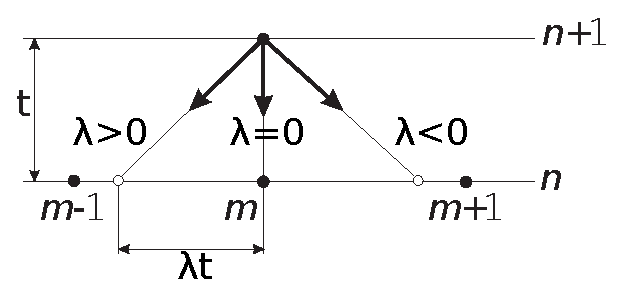
\includegraphics[width=0.3\textwidth]{eps/gcm-idea.eps}}
\caption{Принципиальная схема сеточно-характеристического метода}
\end{figure}
Из точки пересечения характеристики со слоем $n$ значение $v$ переносится в 
точку $\xi^{n+1}_m$:
$$v_i^{n+1}(\xi_m)=v^{n}_i(\xi_m-\lambda_i\tau).$$
Если характеристика не попадает точно в расчётный узел, то применяются различные
методы реконструкции значения в данной точке (в данной работе используется
интерполяция).
\subsubsection{Расчёт граничных узлов}
Метод, описанный в предыдущем пункте, годится лишь для расчёта внутренних узлов
сетки, т.е. только в том случае, если характеристика, выпущенная из узла, не
выводит за пределы области интегрирования. В случае, когда узел является
внешним, применяется иной подход для решения задачи. Рассматриваемая система
уравнений в граничных узлах области интегрирования имеет не больше трёх
\cite{chelnokov} выводящих характеристик, поэтому для корректной постановки
задачи требуется задание граничных условий для каждого внешнего узла сетки в
количестве, равном числу выводящих характеристик. Граничные условия могут быть
нескольких видов (символы без волны -- для первого тела, с волной -- для второго):
\begin{itemize}
\item{свободная граница
\begin{eqnarray}
\sigma_\tau=\sigma_n=0; \nonumber
\end{eqnarray}}
\item{скольжение тел друг относительно друга 
\begin{eqnarray}
v_n=\tilde{v}_n,\nonumber\\
\sigma_n=\tilde{\sigma}_n,\nonumber\\
\sigma_\tau=\tilde{\sigma}_\tau=0; \nonumber
\end{eqnarray}}
\item{слипание тел
\begin{eqnarray}
v_n=\tilde{v}_n,\nonumber\\
v_\tau=\tilde{v}_\tau.
\end{eqnarray}}
\end{itemize}
В случае, когда узел имеет выводящие характеристики, решение определяется
следующим образом: те компоненты искомого вектора $v^T$, которые не имеют
выводящих характеристик, считаются при помощи сеточно"=характеристического
метода, описанного ранее; остальные уравнения заменяются граничными
соотношениями. После этого, решается полученная СЛАУ, из которой определяются
значения всех компонент вектора $v^T$ в текущем узле.

\clearpage
\newpage
\section{Построение параллельной версии}
\subsection{Необходимость}
Однопроцессорная версия алгоритма имеет весьма ограниченную применимость: основным ограничивающим фактором является объём оперативной памяти, доступной на локальном вычислительном узле. Границы применимости однопроцессорной версии можно получить при помощи следующих предположений:
\begin{itemize}
	\item используемые типы данных -- float (4 байта) и int (4 байта);
	\item в каждом узле сетки хранится 3 значения вектора скорости, 6 значений тензора, по 3 значения координат в локальной и подвижной системах, 4 значения параметров реологии среды;
	\item в процессе расчёта каждого временного шага требуется хранить копию расчётов предыдущего временного слоя, для записи результатов на жёсткий диск необходима третья копия;
	\item каждый узел хранит информацию о <<локальной>> топологии сетки для быстрого доступа к соседним тетраэдрам и треугольникам (в среднем по пять значений типа int для каждого типа элементов).
\end{itemize}

Суммарно имеем следующий расход памяти на хранения одного узла: 228 байт. В этих
расчётах не учитываются расходы на хранения топологии всей сетки, ввиду
сложности проведения оценки. Таким образом получаем, что при доступном объёме
памяти в 1 Гб для одного вычислительного узла с максимальной скоростью можно
проводить расчёты на сетках с числом узлов 1-2 миллиона. Под максимальной
скоростью здесь понимается следующее: при расчёте на сетках указанного выше
размера все необходимые данные могут быть полностью помещены в оперативной
памяти, скорость доступ к которой на порядки выше скорости чтения с жёсткого
диска.

Характерный размер сетки для решаемый задачи — \itodo{Посчитать объём точнее}
792000 узлов (11 слоёв, каждый из которых имеет размер 120x120x5). Стоит
отдельно отметить, что размеры этой задачи лежат на самой нижней границе
характерных размеров задач, решение которых представляет практический интерес.
Поставленную задачу уже весьма проблематично решить на одном вычислительном узле
ввиду ограниченного размера доступной для вычислений оперативной памяти.

Другой причиной необходимости создания параллельной версии алгоритма является характер роста вычислительной сложности при увеличении числа узлов сетки ($O(n^3)$). Отсюда следует, что при уменьшении характерных размеров задачи вдвое сложность вычислений возрастает в 8 раз. Очевидно, что задачи такого класса необходимо решать при помощи параллельных версий алгоритмов, чтобы обеспечить хотя бы небольшую масштабируемость.

Таким образом создание параллельной версии алгоритма становится необходимым условием численного моделирования задач подобного рода.

\subsection{Способ построения параллельной версии}
На данный момент существуют два прицинипиально различных подхода к реализации параллельных вычислений:
\begin{itemize}
\item взаимодействие через разделяемую память (shared memory);
\item взаимодействие при помощи обмена сообщениями.
\end{itemize}

Первый метод позволяет <<распараллелить>> алгоритм при помощи минимальных усилий, так как не требует существенных изменений в логике расчёта. Каждый вычислительный узел при таком подходе имеет доступ ко всей памяти, необходимой для расчёта задачи, которая физически находится на \emph{разных} узлах. Таким образом при использовании разделяемой памяти пропадает необходимость синхронизации вычислительных узлов (в смысле пересылок данных), для организации взаимодействия используются различные механизмы захвата управления (к примеру, семафоры или мьютексы). Недостатком такого подхода является чисто техническое ограничение масштабируемости алгоритма: требуется вычислительный кластер с необходимым объёмом оперативной памяти, доступной для работы в разделяемом режиме.

Второй подход требует существенной переработки логики алгоритма, так как необходимо явным образом проводить синхронизацию вычислительных узлов. При этом каждый вычислительный узел использует только доступную локально оперативную память, а всю необходимую информацию запрашивает посредством сообщений во время выполнения. Алгоритмы, построенные по этому принципу, обладают заметно большей масштабируемостью: на данный момент многие вычислительные кластеры имеют более тысячи процессоров.

В данный момент доступ к кластерам, построенным для вычислений с использованием разделяемой памяти, весьма ограничен, доступные же кластеры не обладают необходимым для серьёзного расчёта числом процессоров. Поэтому в основе параллельной версии алгоритма, описываемого в работе, лежит обмен сообщениями между вычислительными узлами. В качестве конкретной реализации этой парадигмы выбран протокол MPI, признанный де-факто стандартом в области высокопроизводительных вычислений.

\subsubsection{Идеи реализации параллельной версии при помощи обмена сообщениями}
Для реализации параллельных вычислений исходная геометрия разбивается на зоны, которые распределяются между вычислительными узлами. Один узел может производить одновременный расчёт нескольких зон. Для обеспечения согласованности расчёта вычислительные узлы обмениваются необходимой информацией о значениях и топологии сеток на границах зон. Для получения максимальной эффективности при параллельном расчёте следует учитывать следующие условия:
\begin{itemize}
	\item для увеличения времени полезного использования кластера необходимо, чтобы время расчёта очередного временного слоя на каждом вычислительном узле было примерно одинаково, так как в противном случае наиболее <<быстрые>> узлы проводят некоторые время в ожидании, при этом не проводя никаких расчётов;
	\item для увеличения скорости синхронизации и расчёта контактных границ крайне желательно, чтобы зоны имели простую геометрию;
	\item граничные части сеток различных зон должны быть построены согласованно (в идеале должны совпадать топологически) для уменьшения потерь точности, связанных с интерполяцией;
	\item расчёт каждого временного слоя должен быть максимально <<параллельным>> в том смысле, что синхронизации происходят редко и согласованно, а данные передаются большими объёмами.
\end{itemize}
\subsubsection{Тестирования производительности MPI}
Для выбора правильных API для построения параллельной версии был проведён ряд тестов производительности обмена сообщениями при помощи MPI. Одним из наиболее важных вопросов, ответ на которых хотелось получить был следующий: каков оптимальный объём сообщения для пересылки? Иными словами, нужно было выяснить, при каких размерах посылаемого сообщения время, затрачиваемое на пересылку одного байта, минимально.
Ниже приведены графики (см. рис. \ref{pic:mpi1host} и рис. \ref{pic:mpi2hosts} зависимости затрат на пересылку одного байта в зависимости от размера сообщения.
\begin{figure}[htp]
\centering
\includegraphics[width=0.8\textwidth]{eps/mpi-1host.eps}
\caption{Затраты на пересылки при использовании одного вычислительного
 узла}
\label{pic:mpi1host}
\end{figure}
\begin{figure}[htp]
\centering
\includegraphics[width=0.8\textwidth]{eps/mpi-2hosts.eps}
\caption{Затраты на пересылки при использовании двух вычислительных узлов}
\label{pic:mpi2hosts}
\end{figure}
Как видно из графиков, для пересылки данных посредством MPI выгодно использовать большие объёмы сообщений. В первую очередь это связано с ростом доли накладных расходов на пересылку сообщения при уменьшении его размера. Другими факторами, снижающими скорость передачи, могут служить буферизация исходящих сообщения, а также блокировки вызывающего процесса при синхронной передаче данных. По результатам проведённых тестов были сделаны следующие выводы;
\begin{itemize}
	\item данные нужно передавать большими объёмами, так как скорость в таких случаях выше;
	\item следует использовать асинхронную передачу данных, возможно, с инициацией приёма до момента посылки данных;
	\item для ускорения процесса синхронизации крайне желательно использовать <<родные>> функции коллективного обмена данными вместо самостоятельной реализации подобного функционала;
	\item следует в полной мере использовать возможности MPI по созданию пользовательских типов данных для уменьшения объёмов памяти, требуемых для хранения временных структур данных, а также для уменьшения временн\'{ы}х затрат на копирование данных внутри вычислительного узла.
\end{itemize}

\subsubsection{Синхронизация шага по времени}
Перед расчётом очередного временного слоя необходимо синхронизировать шаг по времени между всеми вычислительными узлами. В текущей реализации метода с целью увеличения скорости расчёта вводится ограничение на максимально возможный шаг по времени:
\begin{equation}
\label{max_time_step}
\tau_{max}=\frac{h_{min}}{\lambda_{max}},
\end{equation}
где $h_{min}$ -- минимальная высота тетраэдра в сетке, а $\lambda_{max}$ -- максимальное значение коэффициента Ляме в локальной сетке. Так как для расчётов используются неструктурированные тетраэдральные сетки, максимально допустимый шаг по времени может различаться для разных зон. Поэтому в начале расчёта каждого временного слоя вычислительные узлы выбирают максимально допустимый шаг по времени для локальных сеток, после чего из выбирают минимальный из всех полученных. Дальнейший расчёт на всех вычислительных узлах ведётся с одним и тем же шагом по времени. Для выполнения этой операции крайне удобным оказалось использовать встроенную в MPI функцию коллективного обмена:\lstinputlisting[label=lst:time_step_sync,caption=Синхронизация шага по времени]{source/time_step_sync.cpp}
\subsubsection{Синхронизация узлов}
Как было сказано ранее, при параллельных вычисления исходная сетка делится между вычислительными узлами. При этом нередки ситуации, когда одно физическое тело <<разрезано>> на несколько зон. В этом случае получаем следующее: часть узлов, необходимых для расчёта сетки А, принадлежат сетке Б (см. рис. \ref{pic:remote_nodes}). Именно эти узлы (на этапе загрузки они помечаются как REMOTE) необходимо синхронизировать.
\begin{figure}[htp]
\centering
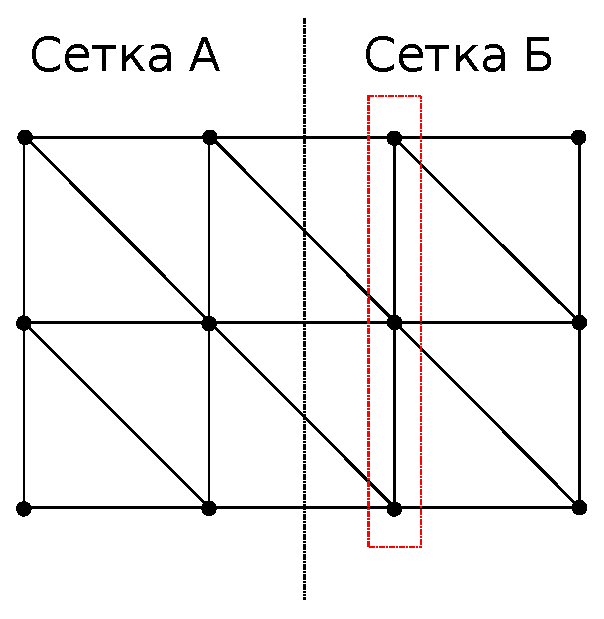
\includegraphics[width=0.4\textwidth]{eps/remote_nodes.eps}
\caption{REMOTE узлы на сетках}
\label{pic:remote_nodes}
\end{figure}
В текущей реализации не используется динамическое перестроение сеток, поэтому на протяжении всего расчёта набор REMOTE узлов не меняется. Это позволяет на этапе загрузки провести первичную обработку сеток, получить список REMOTE узлов для каждой пары сеток и создать пользовательские типы MPI для дальнейших пересылок между вычислительными узлами. Характерный код создания пользовательских типов MPI:
\lstinputlisting[label=lst:custom_types,caption=Создание пользовательских типов MPI]{source/custom_types.cpp}
После этого пересылка всех узлов выполняется так:
\lstinputlisting[label=lst:nodes_sync,caption=Синхронизация REMOTE узлов]{source/nodes_sync.cpp}
\subsubsection{Детектор столкновений}
Для решения поставленной задачи требуется реализовать параллельный алгоритм явного выделения контактных границ. Стандартный подход (именно он использован в этой работе) к реализации состоит из двух этапов:
\begin{itemize}
	\item грубое (см. рис. \ref{pic:collision_detection}) определение областей потенциально возможного контакта при помощи AABB\footnote{AABB (Axis-aligned bounding box) -- ограничивающий параллелепипед, выровненный по осям };
	\item уточнение контактирующих узлов внутри найденных областей.
\end{itemize}
\begin{figure}[htp]
\centering
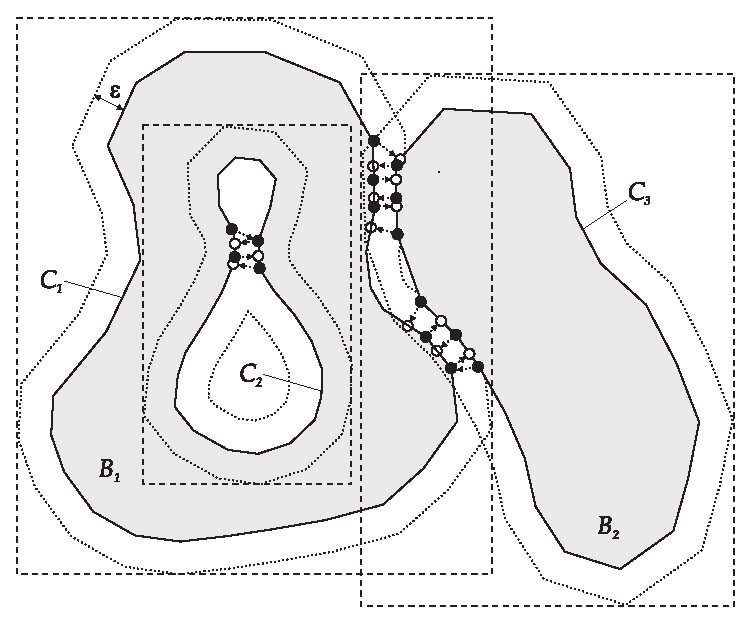
\includegraphics[width=0.6\textwidth]{eps/collision_detection.eps}
\caption{Использование AABB для грубого определения областей контакта. На рисунке изображены тела $B_1$ и $B_2$, а также AABB, построенные для контуров $C_1$ и $C_2$ этих тел. Контакты ищутся в пересечении разных AABB.}
\label{pic:collision_detection}
\end{figure}
Параллельная версия этого алгоритма устроена точно таким же образом. На первом шаге расчёта контактных границ все вычислительные узлы синхронизируют AABB локальных зон, для чего используется вызов стандартной функции MPI:
\lstinputlisting[label=lst:outlines_sync,caption=Синхронизация AABB]{source/outlines_sync.cpp}
После этого каждый вычислительный узел определяет пары <<потенциально>> находящихся в контакте зон -- одной локальной и одной удалённой. Затем для каждой найденной пары проводится уточнение зоны контакта: проверяются <<на контакт>> все пары локальных узлов и удалённых треугольников. Для этого проводится синхронизация треугольников, попавших в зону контакта. Идея здесь схожа с той, что используется при синхронизации удалённых узлов, но имеет некоторые отличия:
\begin{itemize}
	\item т.к. номера треугольников, попавших в зону контакта, заранее не известны, необходимо на первом шаге получить их;
	\item затем, чтобы использовать только одну пересылку на зону контакта, необходимо создать пользовательский тип MPI;
	\item последний шаг -- отправка найденных треугольников получателю.
\end{itemize}
После того, как все треугольники в зоне контакта получены с удалённого вычислительного узла, полным перебором определяются пары <<контактирующих>> узлов и треугольников. Под контактом точки и треугольника здесь понимается следующее: считаем, что треугольник и точка контактируют, если зона влияния (сфера заранее выбранного радиуса) точки пересекает треугольник (см. рис. \ref{pic:contact_detection}).
\begin{figure}[htp]
\centering
\includegraphics[width=0.6\textwidth]{pdf/contact_detection.pdf}
\caption{Определение контакта}
\label{pic:contact_detection}
\end{figure}
Если треугольник и точка находятся в контакте, то следующим шагом нужно построить парный виртуальный узел -- этот узел лежит внутри контактирующего треугольника так, чтобы прямая проходящая через реальный и виртуальный узлы, являлась нормалью к треугольнику (см. рис. \ref{pic:contact_processing}).
\begin{figure}[htp]
\centering
\includegraphics[width=0.6\textwidth]{pdf/contact_processing.pdf}
\caption{Построение виртуальных узлов при обработке контактирующих границ}
\label{pic:contact_processing}
\end{figure}
После того, как виртуальный узел построен, необходимо получить значения всех величин в нём. Для этого в данной работе использовалась линейная интерполяция при помощи барицентрических координат. Задача заключается в следующем (см. рис. \ref{pic:triangle_interpolation}): есть треугольник и точка, лежащая в его плоскости, в трёхмерном пространстве, нужно, используя известные значения в вершинах треугольника, определить значение в в точке.
\begin{figure}[htp]
\centering
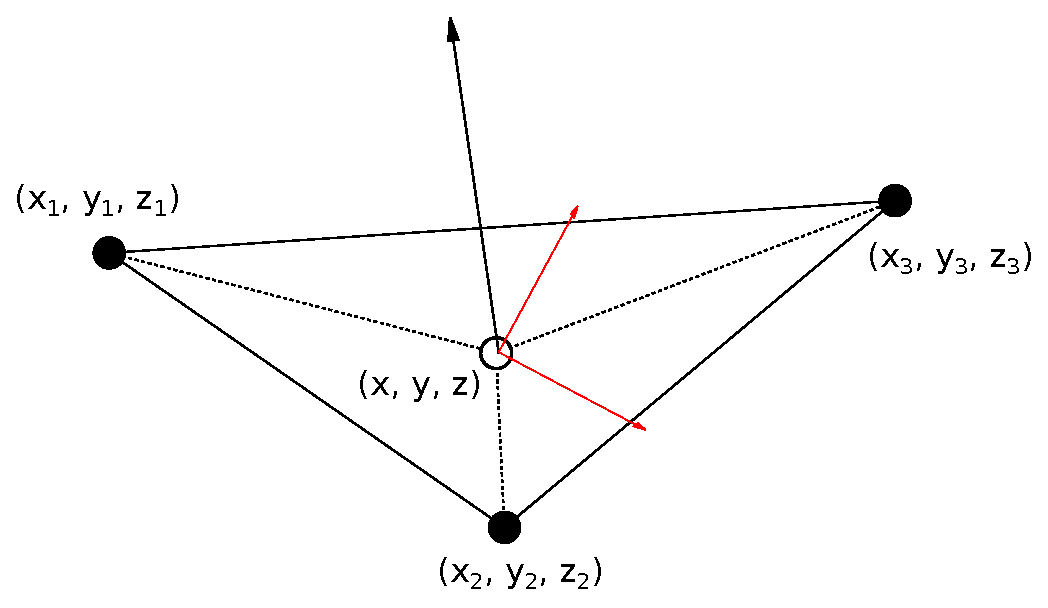
\includegraphics[width=0.6\textwidth]{eps/triangle_interpolation.eps}
\caption{Выбор новых осей координат при интерполяции в треугольнике}
\label{pic:triangle_interpolation}
\end{figure}
В работе используется следующий подход для реализации интерполяции:
\begin{itemize}
	\item поворотом осей координат добиваемся того, чтобы все четыре точки имели одинаковую координату $\tilde{x}$;
	\item используем интерполяцию в плоскости через барицентрические координаты.
\end{itemize}
Пусть $\vec{n}=(n_1,n_2,n_3)$ -- нормаль к плоскости треугольника, тогда в системе координат с базисными векторами:
\begin{eqnarray}
\label{eq:new_coords}
\vec{\tilde{e}}_1=(n_1, n_2, n_3), \nonumber \\
\vec{\tilde{e}}_2=(n_3, 0, -n_1), \nonumber \\
\vec{\tilde{e}}_3=(n_1*n_2, -n_1^2-n_3^2, n_2*n_3)
\end{eqnarray}
все четыре точки имеют одинаковую координату $\tilde{x}$. Такую систему координат невозможно использовать, если $n_1=n_3=0$, но в этом случае все точки имеют одинаковую координату $y$, поэтому сделав замену
\begin{eqnarray}
\label{eq:new_coords_2}
\tilde{x}=y \\
\tilde{y}=x \nonumber \\
\tilde{z}=z
\end{eqnarray}
придём опять к ситуации, когда все четыре точки имеют одинаковую координату $x$.
После этих преобразований значение в точке $(x,y,z)$ может быть вычислено по формуле
\begin{equation}
\label{eq:triangle_interpolation}
v=v_1*\lambda_1+v_2*\lambda_2+v_3*\lambda_3, 
\end{equation}
где $v_1,v_2,v_3$ -- значения в вершинах треугольника, а $\lambda_1,\lambda_2,\lambda_3$ -- барицентрические координаты
\begin{eqnarray}
\label{eq:barycentric_coords}
\lambda_1=\frac{(y_2-y_3)(x-x_3)+(x_3-x_2)(y-y_3)}{(y_2-y_3)(x_1-x_3)+(x_3-x_2)(y_1-y_3)}, \nonumber \\
\lambda_2=\frac{(y_3-y_1)(x-x_3)+(x_1-x_3)(y-y_3)}{(y_2-y_3)(x_1-x_3)+(x_3-x_2)(y_1-y_3)}, \nonumber \\
\lambda_3=1-\lambda_1-\lambda_2.
\end{eqnarray}
Эта интерполяция обладает первым порядком точности, что согласуется с порядком точности остальных частей алгоритма.
\subsubsection{Синхронизация тетраэдров}
Синхронизация тетраэдров необходима для реконструкции локальной топологии сетки, что требуется для правильного расчёта контактной границы. Идеи реализации схожи с теми, что были описаны выше:
\begin{itemize}
	\item вычислительный узел получает список треугольников, для которых нужно синхронизировать тетраэдры;
	\item по списку треугольников строится список тетраэдров, которые необходимо передать удалённому вычислительному узлу;
	\item создаётся пользовательский тип MPI и за одну пересылку осуществляется синхронизация тетраэдров.
\end{itemize}
\subsubsection{Производительность параллельной версии}
Для измерения производительности параллельной версии алгоритма были проведены
расчёты одной и той же тестовой задачи на разном числе вычислительных узлов с
разным способом расчёта контактной границы. В
качестве тестовой задачи была взята задача о распространении волн в 24-слойной
преграде. Каждый слой представляет собой прямоугольный параллелепипед размера
120x120x5 точек. На рисунках \ref{pic:gcm_boost} и
\ref{pic:gcm_efficiency} представлены зависимости производительности и
эффективности от числа используемых вычислительных узлов.
\begin{figure}[htp]
\centering
\includegraphics[width=\textwidth]{eps/gcm3d-boost.eps}
\caption{Зависимость производительности от количества вычислительных узлов}
\label{pic:gcm_boost}
\end{figure}
\begin{figure}[htp]
\centering
\includegraphics[width=\textwidth]{eps/gcm3d-efficiency.eps}
\caption{Зависимость эффективности использования кластера от количества вычислительных узлов}
\label{pic:gcm_efficiency}
\end{figure}

Как видно из графиков, использование сквозного счёта даёт практически линейный
рост производительности с эффективным временем использования кластера в $\sim
90\%$.
Расчёт с явным выделением контакта даёт производительность в $\sim30\%$. Это  в
первую очередь связано с очень большой площадью контактирующих поверхностей. Так, в тестовом
примере $\sim 40\%$ узлов исходной сетки принимают участие в расчёте контакта.
При этом распределение контактирующих поверхностей по вычислительным узлам
неоднородно: слои, находящиеся <<в центре>> имеют по две контактирующих
поверхности, а <<крайние>> слои лишь по одной.

Полученные характеристики производительности следует воспринимать как оценочные
для верхней и нижней границ. Соответственно, ожидаемая эффективность при расчёте
реальных задач должна составить $\sim 60\%$. Этот результат является вполне
приемлемым, так как позволяет обеспечить расчёт больших областей с высокой
точностью при разумном КПД.

\clearpage
\newpage
\section{Полученные результаты}
\subsection{Задача о сферическом взрыве}
Проверка корректности работы разработанного алгоритма проводилась при помощи численного решения задачи о сферическом взрыве.
\subsection{Волновая картина в субпакете}

\clearpage
\newpage
\section{Заключение}
Результаты, полученные в результате выполнения дипломного проекта:
\begin{itemize}
\item предложена схема построения параллельной версии
сеточно-характеристического метода для решения задач механики деформируемого
твёрдого тела в случае трёх пространственных переменных;
\item реализована предложенная схема в виде программного комплекса для
высокопроизводительных вычислений;
\item проведено тестирования масштабируемости параллельной версии алгоритма;
\item рассчитан ряд тестовых задач для подтверждения корректности реализации;
\item численно смоделирована задача о непробивающем ударе многослойной
конструкции и качественно получена волновая картина в материале.
\end{itemize}

\clearpage
\newpage
\begin{thebibliography}{99}
\addcontentsline{toc}{section}{Литература}
\bibitem{novatsky}\todo{Оформить библиографию правильно}Новацкий В. К. Теория упругости. — М. : Мир, 1975.
\bibitem{sedov}Седов Л. И. Механика сплошной среды. — М. : Наука, 1970.
\bibitem{belocerkovsky}Белоцерковский О.М. Численное моделирование в механике
сплошных сред. — М.: Физико-математическая литература. 1994, 442 с.
\bibitem{magomedov}Магомедов К.М., Холодов А.С. Сеточно-характеристические
численные методы. — М.: Наука, 1988, 288 с.
\bibitem{holodov}Холодов А.С., Холодов Я.А. О критериях монотонности разностных
схем для уравнений гиперболического типа. 
\bibitem{chelnokov}Челноков Ф.Б. Численное моделирование деформационных
процессов в средах со сложной структурой.
\bibitem{fedorenko}Федоренко Р.П. Введение в вычислительную физику. М.:
Изд-во Моск. физ. -техн. ин-та, 1994, 528 с 
\end{thebibliography}

\end{document}
